\section{Obiettivo}
Il problema dello zaino multidimensionale (Multidimensional Knapsack Problem) è
un'estensione del più noto problema dello Zaino. L'obbiettivo è sempre lo
stesso, trovare un set di oggetti che massimizzi il profitto totale facendo in
modo di non superare la capienza massima dello zaino, solo con l'aggiunta di più
vincoli: non dovremmo solo preoccuparci della capienza dello zaino ma anche di
altri $n$ differenti fattori.\\

Questo problema può essere formalmente sintetizzato come segue:

\[
    \max \sum_{j=1}^{n} p_j x_j
\]

\[
    \text{subject to: } \sum_{j=1}^{n} r_{i,j} x_j \leq b_i, \ \ i = 1,2,\ldots, m
\]

con $x_j = \{0, 1\}$, $n$ il numero di oggetti, $m$ il numero di vincoli, $b$ il limite massimo per ogni vincolo,
$r$ il valore per ogni singolo vincolo di ogni oggetto.

\section{Istanze del Problema}

L'algoritmo per la risoluzione di questo problema verrà testato utilizzando il dataset
\href{http://people.brunel.ac.uk/~mastjjb/jeb/orlib/mknapinfo.html}{OR-Library}: una
raccolta di varie istanze, di differenti dimensioni, per una svariata moltitudine di
problemi. Una singola istanza si presenta come segue:

\begin{lstlisting}[caption={Esempio di Istanza di un problema MKP con 6 oggetti e 10 vincoli.}]
6
100,600,1200,2400,500,2000
10
8,12,13,64,22,41
8,12,13,75,22,41
3,6,4,18,6,4
5,10,8,32,6,12
5,13,8,42,6,20
5,13,8,48,6,20
0,0,0,0,8,0
3,0,4,0,8,0
3,2,4,0,8,4
3,2,4,8,8,4
80,96,20,36,44,48,10,18,22,24
3800
\end{lstlisting}

La prima riga contiene il numero di oggetti, la seconda il valore di ogni singolo
oggetto, la terza il numero di parametri, le successive righe rappresentano i
valori dei coefficienti del primo parametro, del secondo e così via fin quando non si raggiunge il
numero di parametri. La penultima riga indica il valore massimo per ogni parametro (rappresenta quindi
il vincolo che non si può superare) e
l'ultima il valore della soluzione ottimale.

\begin{table}[H]
    \centering
    \begin{tabular}{||c||c||c||c||c||c||c||c||c||c||c||c||}
        \textbf{ID} & \textbf{f0} & \textbf{f1} & \textbf{f2} & \textbf{f3} & \textbf{f4} & \textbf{f5} & \textbf{f6} & \textbf{f7} & \textbf{f8} & \textbf{f9} & \textbf{Value} \\
        \hline
        0           & 8.0         & 8.0         & 3.0         & 5.0         & 5.0         & 5.0         & 0.0         & 3.0         & 3.0         & 3.0         & 100.0          \\
        1           & 12.0        & 12.0        & 6.0         & 10.0        & 13.0        & 13.0        & 0.0         & 0.0         & 2.0         & 2.0         & 600.0          \\
        2           & 13.0        & 13.0        & 4.0         & 8.0         & 8.0         & 8.0         & 0.0         & 4.0         & 4.0         & 4.0         & 1200.0         \\
        3           & 64.0        & 75.0        & 18.0        & 32.0        & 42.0        & 48.0        & 0.0         & 0.0         & 0.0         & 8.0         & 2400.0         \\
        4           & 22.0        & 22.0        & 6.0         & 6.0         & 6.0         & 6.0         & 8.0         & 8.0         & 8.0         & 8.0         & 500.0          \\
        5           & 41.0        & 41.0        & 4.0         & 12.0        & 20.0        & 20.0        & 0.0         & 0.0         & 4.0         & 4.0         & 2000.0         \\
    \end{tabular}
    \caption{Rappresentazione sotto forma tabellare dell'istanza precedente}
\end{table}

\section{Implementazione}

Il problema descritto in precedenza verrà risolto mediante l'implementazione
di un Algoritmo Genetico. È stato scelto questo approccio per la sua
semplicità di implementazione e relativa velocità di esecuzione. Di seguito
saranno descritte le principali componenti che caratterizzano questo algoritmo.
% Vedremo come sarà necessario l'utilizzo di un operatore di 'riparazione' (repair operator)

\subsection{Initial Population}
La prima operazione per l'implementazione di un algoritmo genetico è quella di
andare a generare la popolazione iniziale. In questa implementazione verrà
fatto in maniera casuale applicando una strategia che permetterà di creare
elementi della popolazione (noti anche come \textit{cromosomi}) sempre ammissibili.
Questa operazione può essere descritta come segue:

\begin{enumerate}
    \item Crea una soluzione temporanea vuota (nessun oggetto),
    \item Estrai casualmente un oggetto tra quelli disponibili, \label{enum:loop}
    \item Prova ad aggiungere questo oggetto alla soluzione temporanea, \label{enum:check}
          \begin{itemize}
              \item se è possibile farlo: \begin{itemize}
                        \item aggiungi l'oggetto definitivamente alla soluzione,
                        \item rimuovi l'oggetto dagli oggetti disponibili,
                        \item continua dal punto \ref{enum:loop}.
                    \end{itemize}
              \item se non lo è: \begin{itemize}
                        \item aggiungi la soluzione creata alla lista delle
                              soluzioni generate fin ora.
                    \end{itemize}
          \end{itemize}
    \item Continua fin quando non è stato generato il numero desiderato di soluzioni.
\end{enumerate}

\begin{minipage}{\textwidth}
    \begin{lstlisting}
PROCEDURE initialize_population
    INPUT:
        num_elem: number of solution to generate
        item_list: list of items
        num_items: number of items
        W: constraints upper bound

    population <- empty list of Solutions
    f_obj <- list of zeros with length num_elem

    FOR i <- 0 TO num_elem - 1 DO
        tmp_sol <- list of zeros with length num_items

        // list of item indexes
        T <- list of integers from 0 to num_items - 1

        R <- list of zeros with length equal to the
             number of constraints in the problem

        j <- randomly select an integer from T
        item <- item_list.pop(j)

        WHILE all elements of (R + item) <= W DO
            tmp_sol[j] <- 1
            R <- R + item

            IF length(T) <= 0 THEN
                EXIT WHILE loop
            END IF

            j <- randomly select an integer from T
            item <- item_list.pop(j)
        END WHILE

        APPEND tmp_sol to population
        f_obj[i] <- calculate the objective function value for tmp_sol
    END FOR
END PROCEDURE
\end{lstlisting}
    \captionof{lstlisting}{Pseudocodice per la Selezione della Popolazione iniziale.}
\end{minipage}\\

Possiamo notare come nel punto \ref{enum:check}, grazie alle operazioni
descritte, ogni soluzione generata sarà sicuramente ammissibile perchè verrà
sempre controllato che, ogni qualvolta viene aggiunto un oggetto, la nuova
soluzione non superi i limiti massimi imposti al problema.

\subsection{Mating Pool Selection}
Una volta descritto come inizializzare la popolazione, và specificato come
selezionare gli individui per formare il Mating Pool, un insieme di $N/2$ coppie
che verranno utilizzate al passaggio successivo: \textbf{Crossover}. La
selezione del Mating Pool può avvenire in due modi: tramite \textit{Roulette
    Wheel} o \textit{Tournaments}. Per la semplicità di implementazione e
soprattutto per il basso costo computazionale è stato implementato il metodo
basato sui Tornei. Vengono selezionati casualmente un numero $k$ di elementi
della popolazione e tra questi viene preso il cromosoma con valore di fitness
più alto. Tramite questa operazione vengono generate $N/2$ coppie che poi verranno
passate all'operatore di Crossover.
Di seguito lo pseudocodice che riassume questa operazione.

\begin{lstlisting}[caption={Implementazione del metodo per la selezione del Mating Pool basata sui Tornei.}]
FUNCTION tournament(k: INTEGER) RETURNS Solution
    random_select_solutions <- select k solution from population randomly

    max_index <- select the index of solution with max fitness value
                in random_select_solutions

    RETURN population[max_index]
END FUNCTION

PROCEDURE select_mating_pool
    INPUT:
        population: List of all chromosomes (solutions)
        k: tournament parameter

    mating_pool <- empty list

    FOR i <- 1 TO LENGTH(population) // 2 DO
        c1 <- tournament(k)
        c2 <- tournament(k)

        APPEND (c1, c2) to mating_pool
    END FOR

    RETURN mating_pool
END PROCEDURE
\end{lstlisting}

\subsection{Crossover Operator}
L'operatore di Crossover prende gli elementi del Mating Pool e genera un nuovo
elemento chiamato \textit{figlio}. Questo è un \textbf{Crossover Uniforme}: dati
due cromosomi, che prendono il nome di \textit{padri} (indicati con $s_1$ e
$s_2$), viene generato un nuovo individuo figlio che eredita in modo uniforme i
geni dai due padri. Il crossover viene eseguito con una probabilità data dal
parametro \verb|pcross|. Di seguito lo pseudocodice.

\begin{minipage}{\textwidth}
    \begin{lstlisting}
FUNCTION uniform_crossover_operator(s1, s2) RETURNS Solution
    c = ARRAY OF ZEROS with length LENGTH(s1)

    FOR i <- 1 TO LENGTH(s1) DO
        IF RANDOM_BOOLEAN() THEN
            c[i] <- s1[i]
        ELSE
            c[i] <- s2[i]
        END IF
    END FOR

    RETURN c
END FUNCTION

PROCEDURE do_crossover
    INPUT:
        mating_pool: N/2 couples from Selecting Mating Pool Phase
        pcross: Crossover probability

    children <- empty list

    FOR EACH (s1, s2) IN mating_pool DO
        IF RANDOM_FLOAT() < pcross THEN
            c <- uniform_crossover_operator(s1, s2)
            APPEND c to children
        ELSE
            APPEND s1 to children
            APPEND s2 to children
        END IF
    END FOR

    RETURN children
END PROCEDURE
\end{lstlisting}
    \captionof{lstlisting}{Implementazione dell'operatore di Crossover.}
\end{minipage}

\subsection{Mutation Operator}

L'operatore di Mutazione è il responsabile di alterare i geni dei cromosomi
risultanti dalla precedente fase di Crossover (indipendentemente se sono
genitori o figli). In base al parametro \verb|pmut| (\textit{mutation
    probability}), per ogni gene di ogni cromosoma, viene scelto se effettuare una
mutazione oppure no. La mutazione consiste nel cambiare il rispettivo gene
scelto tramite una semplice operazione di negazione.

\begin{minipage}{\textwidth}
    \begin{lstlisting}
PROCEDURE do_mutation
    INPUT:
        children: Crossover Phase Result
        pmut: Mutation Probability

    FOR EACH child in children DO
        FOR i <- 0 TO LENGTH(child) - 1 DO
            IF RANDOM_FLOAT() < pmut THEN
                child[i] <- not child[i]
            END IF
        END FOR
    END FOR
END PROCEDURE
\end{lstlisting}
    \captionof{lstlisting}{Pseudocodice dell'operatore di Crossover.}
\end{minipage}

\subsection{Repair Operator}

Una volta terminata la fase di Mutazione, abbiamo in output una serie di
cromosomi figli che molto probabilmente non rispettano i criteri del problema e
non sono quindi soluzioni ammissibili. C'è la necessità quindi di andare a
\textquote*{riparare} ogni cromosoma che porti ad una soluzione non valida.
L'operatore che si occupa di questa procedura è stato implementato in 2 fai: la
prima \textbf{Sottrattiva} e la seconda \textbf{Additiva}. L'idea che c'è dietro
a questa procedura può essere riassunta come segue:

\begin{enumerate}
    \item Per ogni figlio controlla se è una soluzione ammissibile.
          \label{enum:looprep}
    \item Se lo è, torna al punto \ref{enum:looprep}
    \item Altrimenti:
          \begin{enumerate}
              \item \textbf{Fase Sottrattiva}: rimuovi un oggetto alla volta
                    dalla soluzione, fin quando la soluzione non diventa ammissibile
              \item \textbf{Fase Additiva}: aggiungi un oggetto alla volta alla
                    soluzione, fin quando è possibile (fin quando la soluzione
                    rimane ancora ammissibile).
              \item Torna al punto \ref{enum:looprep}
          \end{enumerate}
\end{enumerate}

Durante le due fasi, gli oggetti vengo scelti in modo ordinato in base ad un
parametro chiamato \textit{Importanza}. L'idea di base è di rimuovere prima gli
oggetti meno importanti e di aggiungere poi quelli più importanti. Questo parametro
viene calcolato in base alla seguente formula:

\begin{equation}\label{eq:importance}
    Importance(j) = \frac{\sum_{i=1}^{m} r_{i,j} b_i}{\sum_{i=1}^{m} b_i} \frac{1}{p_j}
\end{equation}

\begin{minipage}{\textwidth}
    \begin{lstlisting}{mathescape=true}
PROCEDURE repair_operator
    INPUT:
        children: Mutation Phase Result

    sorted_objects <- sort object according to equation $\text{\ref{eq:importance}}$
    sorted_index <- get indexes of sorted object by Importance

    FOR EACH child in children DO
        IF child is feasible solution DO
            continue
        END IF

        // DROP PHASE
        child <- remove object from child, starting from less Important,
                until child is feasible solution

        // ADD PHASE
        child <- add object to child, starting from most Important,
                until child is feasible solution
    END FOR
END PROCEDURE
    \end{lstlisting}
    \captionof{lstlisting}{Pseudocodice dell'operatore di Riparazione.}
\end{minipage}

\subsection{Select New Population}

Una volta completata la fase di Riparazione e quindi con un'insieme di soluzioni
sicuramente accettabili, và selezionata la nuova popolazione da passare alla
generazione successiva dell'algoritmo genetico. Per farlo è stata implementata
la strategia in cui \textit{sopravvivono i migliori} (un caso particolare
dell'elitismo). In questa fase vengono scelti i migliori individui, in base alla
fitness, della popolazione indipendentemente se sono \textquote*{figli} o
\textquote*{genitori} (non conta quindi l'età).

\begin{minipage}{\textwidth}
    \begin{lstlisting}
PROCEDURE select_new_population
    INPUT:
        population: Actual population
        children: Repair Phase Result
        num_elem: max population length

    total_solutions <- population + children
    total_fitnesses <- compute fitness value for all total_solutions

    total_solutions <- sort by fitness value (desc)
    total_fitnesses <- sort by fitness value (dec)

    population <- total_solutions[0...num_elem]
    fitnesses <- total_fitnesses[0...num_elem]
END PROCEDURE
\end{lstlisting}
    \captionof{lstlisting}{Pseudocodice della fase di selezione della nuova popolazione.}
\end{minipage}

\section{Stima dei Parametri}

Il punto cruciale quando si esegue un algoritmo genetico è l'individuazione dei
vari parametri che lo caratterizzano.

\begin{itemize}
    \item \verb|pcross| (\textit{Crossover Probability}): probabilità di
          effettuare il crossover di un elemento del Mating Pool (generalmente è
          elevata),
    \item \verb|pmut| (\textit{Mutation Probability}): probabilità di mutare un
          singolo gene di un elemento dell'insieme dei figli generato dalla fase
          di Crossover (generalmente è bassa),
    \item \verb|ngen| (\textit{Max Generation Number}): numero di Generazioni
          dopo il quale l'algoritmo si ferma,
    \item \verb|plen| (\textit{Population Length}): lunghezza della popolazione,
    \item \verb|tk| (\textit{Tournaments k}): massimo numero di elementi tra cui
          scegliere il migliore durante i tornei.
\end{itemize}

Per la stima di quest'ultimi è stato selezionato un dataset di \textit{Tuning},
composto da 11 istanze più o meno grandi, che meglio rappresentavano il dataset
di tutte le istanze a disposizione. In questo dataset abbiamo una varietà di
istanze molto vasta, possiamo trovarne alcune che hanno 6 oggetti e 10 parametri
fino ad altre con oltre i 100 oggetti. Di seguito una tabella riassuntiva.

\begin{table}[H]
    \centering
    \begin{tabular}{||c||c||c||}
        \textbf{file}    & \textbf{Oggetti} & \textbf{Parametri} \\
        \hline
        \verb|MKP01.txt| & 6                & 10                 \\
        \verb|MKP03.txt| & 15               & 10                 \\
        \verb|MKP05.txt| & 28               & 10                 \\
        \verb|MKP07.txt| & 50               & 5                  \\
        \verb|MKP11.txt| & 28               & 2                  \\
        \verb|MKP17.txt| & 105              & 2                  \\
        \verb|MKP21.txt| & 30               & 5                  \\
        \verb|MKP23.txt| & 40               & 5                  \\
        \verb|MKP33.txt| & 60               & 5                  \\
        \verb|MKP41.txt| & 80               & 5                  \\
        \verb|MKP47.txt| & 90               & 5
    \end{tabular}
    \caption{Contenuto del dataset di Tuning.}
\end{table}

Per ogni file nel dataset è stato eseguito l'algoritmo 5 volte e sono stati
salvati i risultati: nome del file, soluzione trovata (\textit{found}),
soluzione originale (\textit{target}), un bit per indicare il successo e la
differenza tra \textit{target} e \textit{found}. Sono stati poi scelti altri
parametri e rieseguita la fase di tuning.
Per ogni esecuzione della fase di tuning si ottiene un file di
questo tipo:\\

\begin{minipage}{\textwidth}
    \begin{lstlisting}
,file,gen,found,target,success,diff
0,data/MKP01.txt,52,3800.0,3800.0,True,0.0
1,data/MKP01.txt,1,3800.0,3800.0,True,0.0
2,data/MKP01.txt,0,3800.0,3800.0,True,0.0
3,data/MKP01.txt,48,3800.0,3800.0,True,0.0
4,data/MKP01.txt,87,3800.0,3800.0,True,0.0
5,data/MKP03.txt,20,3915.0,4015.0,False,100.0
\end{lstlisting}
    \captionof{lstlisting}{File risultante da una esecuzione della fase di Tuning.}
\end{minipage}\\

Sono stati selezionati i seguenti parametri e utilizzati per eseguire la fase di
Tuning.

\begin{table}[H]
    \centering
    \begin{tabular}{||c||c||c||c||c||}
        \textbf{pmut} & \textbf{pcross} & \textbf{ngen} & \textbf{plen} & \textbf{tk} \\
        \hline
        0.01          & 0.90            & 100           & 16            & 5           \\
        0.02          & 0.97            & 250           & 40            & 31          \\
        0.02          & 0.97            & 250           & 80            & 40          \\
        0.02          & 0.97            & 250           & 100           & 40          \\
        0.03          & 0.97            & 250           & 71            & 33          \\
        0.05          & 0.97            & 250           & 20            & 7           \\
        0.05          & 0.97            & 250           & 40            & 31          \\
        0.05          & 0.97            & 250           & 100           & 61          \\
        0.05          & 0.99            & 250           & 20            & 16          \\
        0.05          & 0.99            & 250           & 80            & 50          \\
        0.05          & 0.99            & 250           & 100           & 80
    \end{tabular}
    \caption{Lista dei parametri scelti per essere utilizzati nella fase di Tuning.}
\end{table}

Per ogni esecuzione poi sono stati generati 2 grafici: il primo ci mostra la
differenza media, in percentuale, tra \textit{target} e \textit{found}; il
secondo il numero di successi e fallimenti per ogni file.

\begin{figure}[H]

    \centering
    \begin{subfigure}{.3\textwidth}
        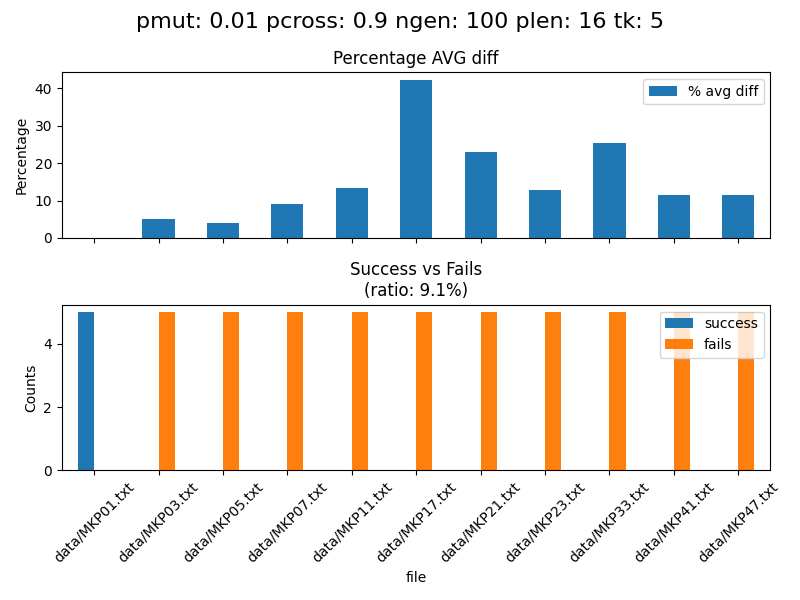
\includegraphics[width=\textwidth]{img/tuning/tuning_results_1_90_100_16_5.png}
    \end{subfigure}
    \begin{subfigure}{.3\textwidth}
        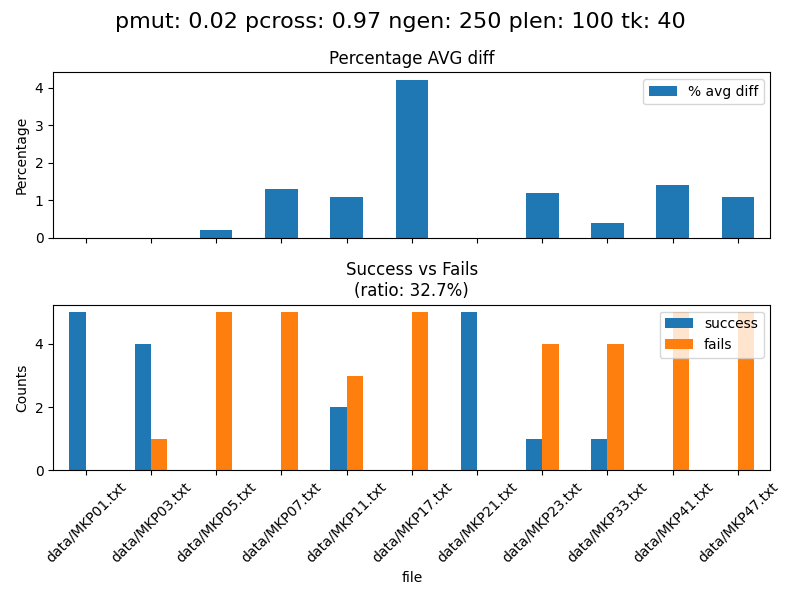
\includegraphics[width=\textwidth]{img/tuning/tuning_results_2_97_250_100_40.png}
    \end{subfigure}
    \begin{subfigure}{.3\textwidth}
        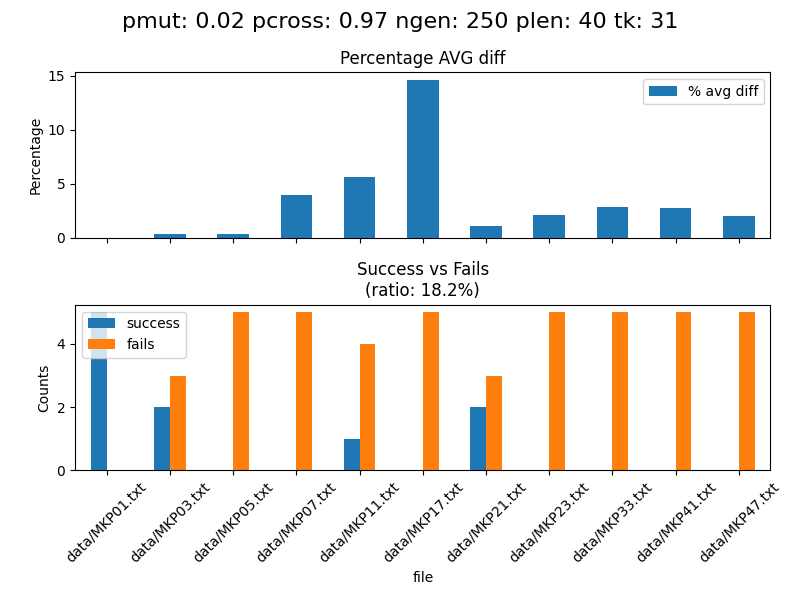
\includegraphics[width=\textwidth]{img/tuning/tuning_results_2_97_250_40_31.png}
    \end{subfigure}\\

    \begin{subfigure}{.3\textwidth}
        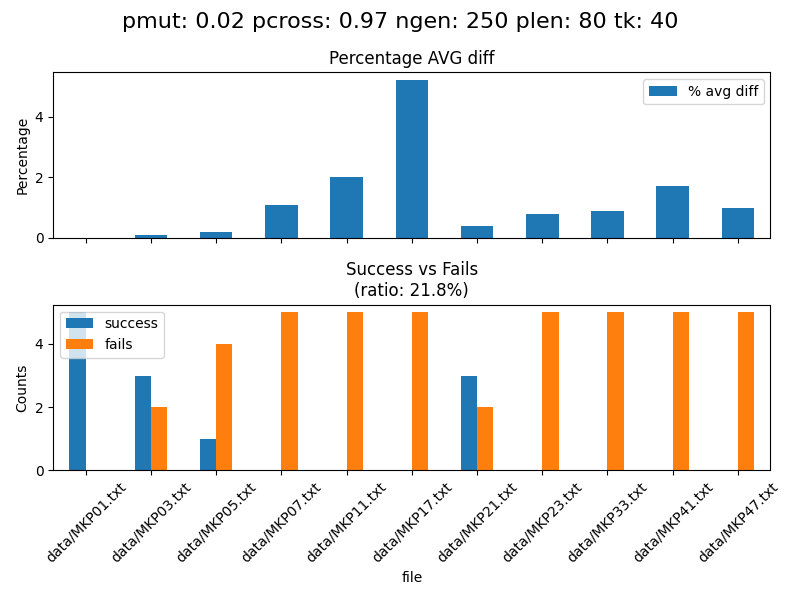
\includegraphics[width=\textwidth]{img/tuning/tuning_results_2_97_250_80_40.png}
    \end{subfigure}
    \begin{subfigure}{.3\textwidth}
        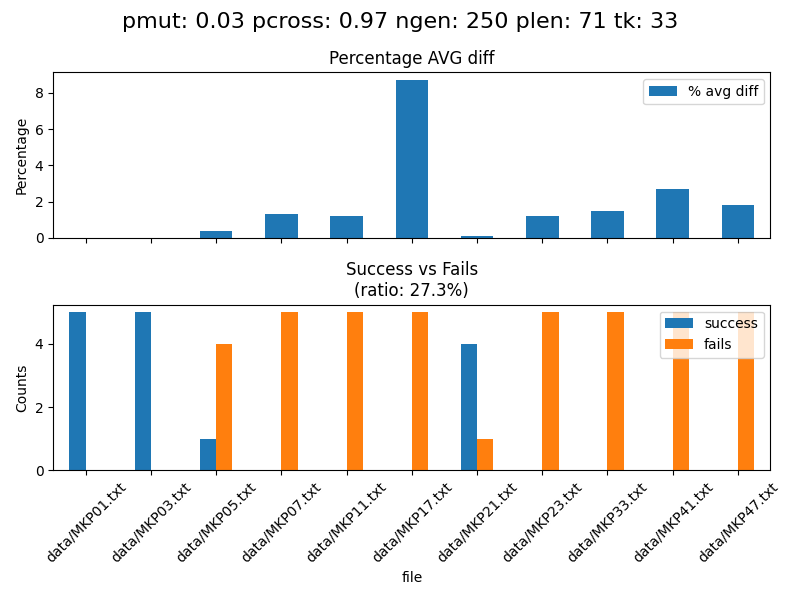
\includegraphics[width=\textwidth]{img/tuning/tuning_results_3_97_250_71_33.png}
    \end{subfigure}
    \begin{subfigure}{.3\textwidth}
        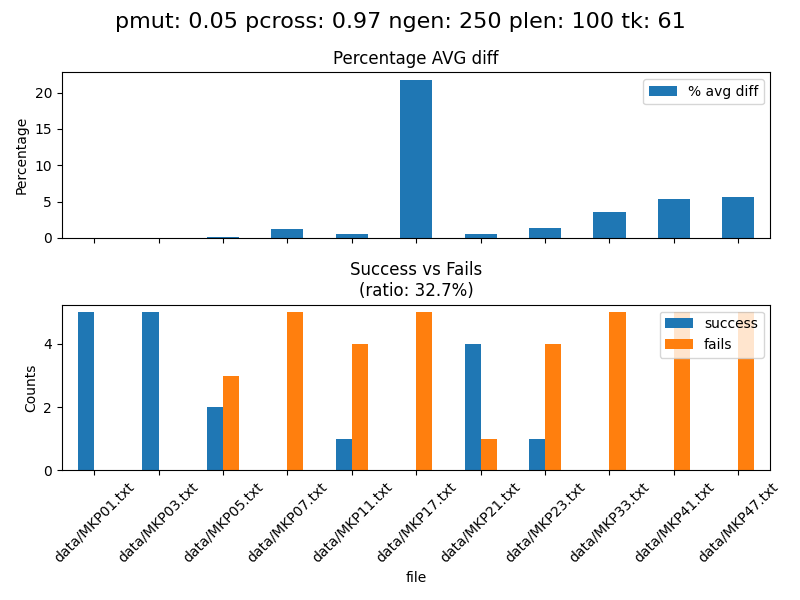
\includegraphics[width=\textwidth]{img/tuning/tuning_results_5_97_250_100_61.png}
    \end{subfigure}\\

    \begin{subfigure}{.3\textwidth}
        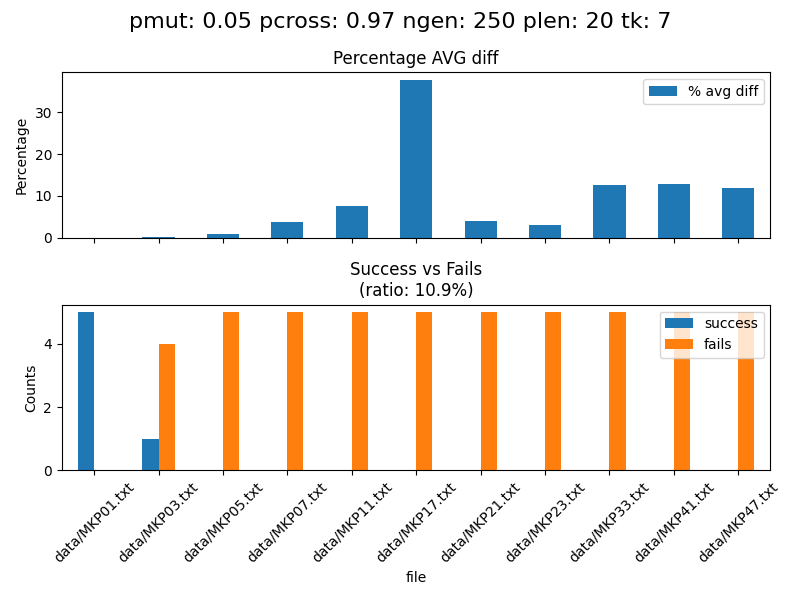
\includegraphics[width=\textwidth]{img/tuning/tuning_results_5_97_250_20_7.png}
    \end{subfigure}
    \begin{subfigure}{.3\textwidth}
        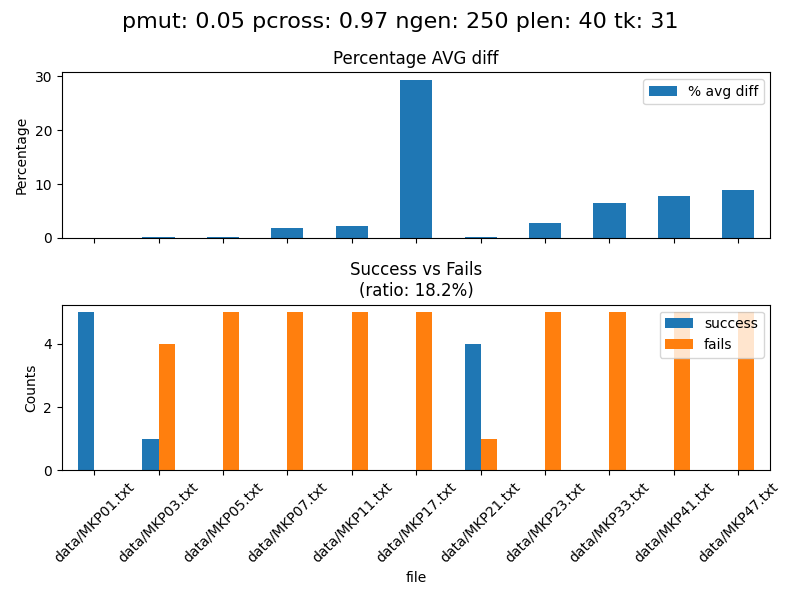
\includegraphics[width=\textwidth]{img/tuning/tuning_results_5_97_250_40_31.png}
    \end{subfigure}
    \begin{subfigure}{.3\textwidth}
        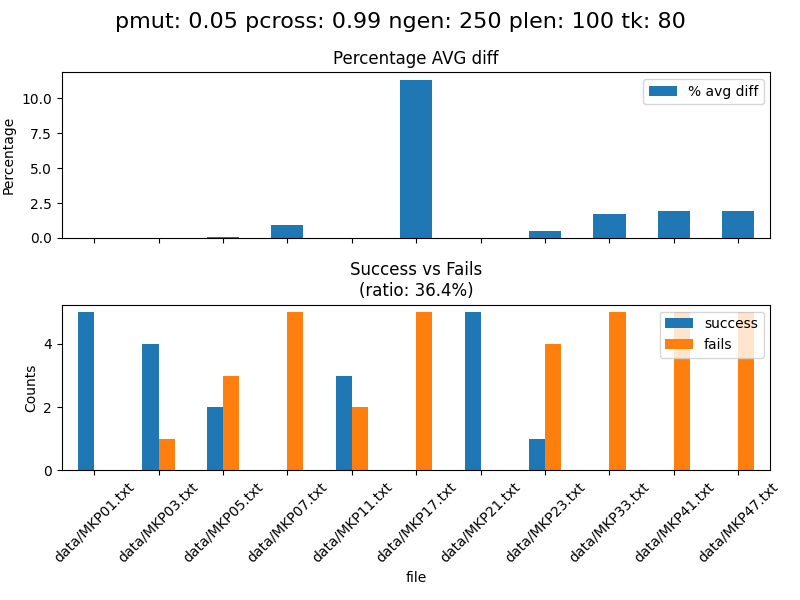
\includegraphics[width=\textwidth]{img/tuning/tuning_results_5_99_250_100_80.png}
    \end{subfigure}\\

    \begin{subfigure}{.3\textwidth}
        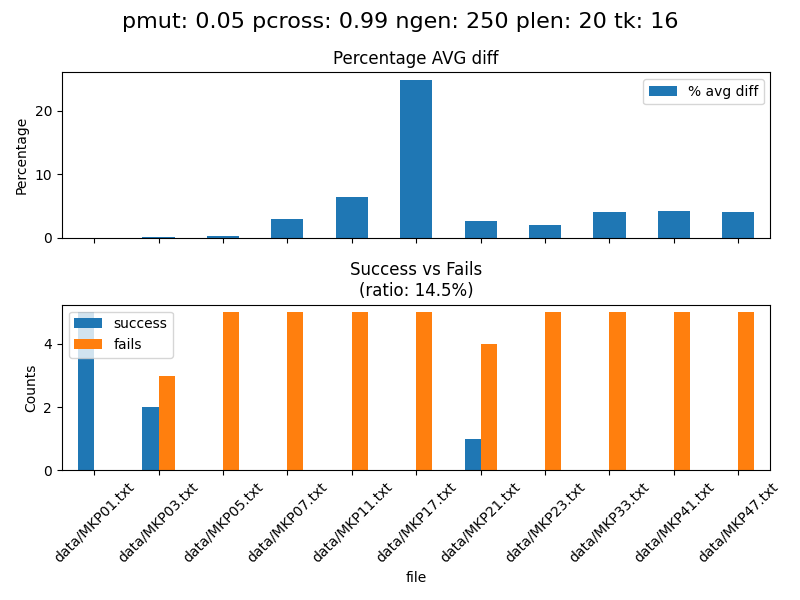
\includegraphics[width=\textwidth]{img/tuning/tuning_results_5_99_250_20_16.png}
    \end{subfigure}
    \begin{subfigure}{.3\textwidth}
        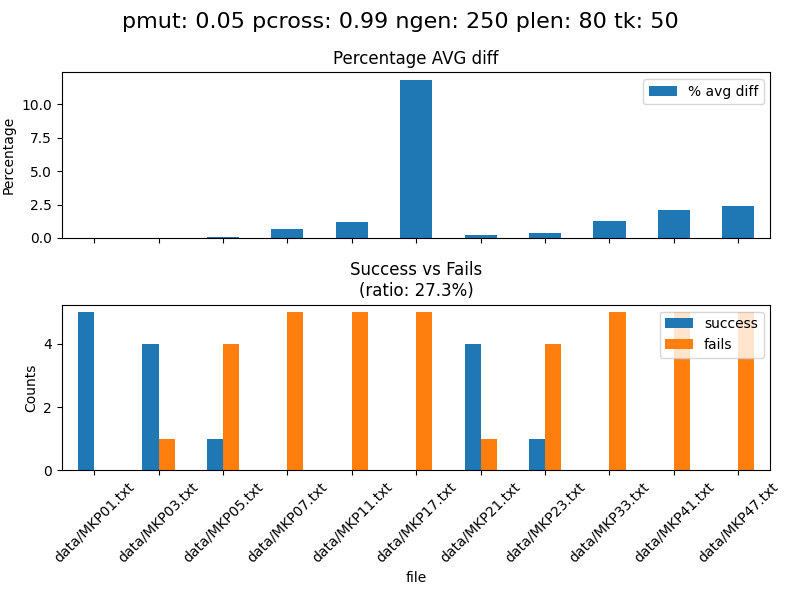
\includegraphics[width=\textwidth]{img/tuning/tuning_results_5_99_250_80_50.png}
    \end{subfigure}

    \caption{Grafici ottenuti dalla fase di Tuning.}
\end{figure}

Dai precedenti grafici si possono individuare i 3 migliori set di parametri che
verranno utilizzati nella successiva fase di Valutazione delle Performance.

\begin{table}[H]
    \centering
    \begin{tabular}{||c||c||c||}
        \textbf{Parameters}                           & \textbf{Success Ratio (\%)} & \textbf{Max AVG Diff (\%)} \\
        \hline
        pmut 0.05;pcross 0.99;ngen 250;plen 100;tk 80 & 36.4                        & 12.0                       \\
        pmut 0.02;pcross 0.97;ngen 250;plen 100;tk 40 & 32.7                        & 5.0                        \\
        pmut 0.05;pcross 0.97;ngen 250;plen 100;tk 61 & 32.7                        & 21.0                       \\
    \end{tabular}
    \caption{Top 3 set di parametri individuati nella fase di Tuning.\label{tab:param}}
\end{table}

\section{Valutazione delle Performance}

Infine, dopo aver individuato i 3 set di parametri che performano meglio, è
stato scelto un dataset di \textit{Testing} su cui testare le scelte della fase
precedente.

\begin{table}[H]
    \centering
    \begin{tabular}{||c||c||c||}
        \textbf{file}    & \textbf{Oggetti} & \textbf{Parametri} \\
        \hline
        \verb|MKP02.txt| & 10               & 10                 \\
        \verb|MKP04.txt| & 20               & 10                 \\
        \verb|MKP06.txt| & 39               & 5                  \\
        \verb|MKP08.txt| & 60               & 30                 \\
        \verb|MKP10.txt| & 28               & 2                  \\
        \verb|MKP12.txt| & 28               & 2                  \\
        \verb|MKP20.txt| & 30               & 5                  \\
        \verb|MKP22.txt| & 30               & 5                  \\
        \verb|MKP24.txt| & 40               & 5                  \\
        \verb|MKP30.txt| & 50               & 5                  \\
        \verb|MKP36.txt| & 70               & 5                  \\
        \verb|MKP40.txt| & 80               & 5                  \\
        \verb|MKP46.txt| & 90               & 5                  \\
        \verb|MKP48.txt| & 27               & 4                  \\
        \verb|MKP50.txt| & 29               & 2                  \\
        \verb|MKP54.txt| & 28               & 4                  \\
    \end{tabular}
    \caption{Contenuto del dataset di Testing.}
\end{table}

Similmente alla fase di Tuning, per ogni elemento del dataset di Testing è stato
eseguito l'algoritmo genetico 10 volte, utilizzando i parametri della Tabella
\ref{tab:param} e salvando sempre i risultati come in precedenza.
I risultati finali sono riassunti dai seguenti grafici.


\begin{figure}[H]
    \centering
    \begin{subfigure}{.49\textwidth}
        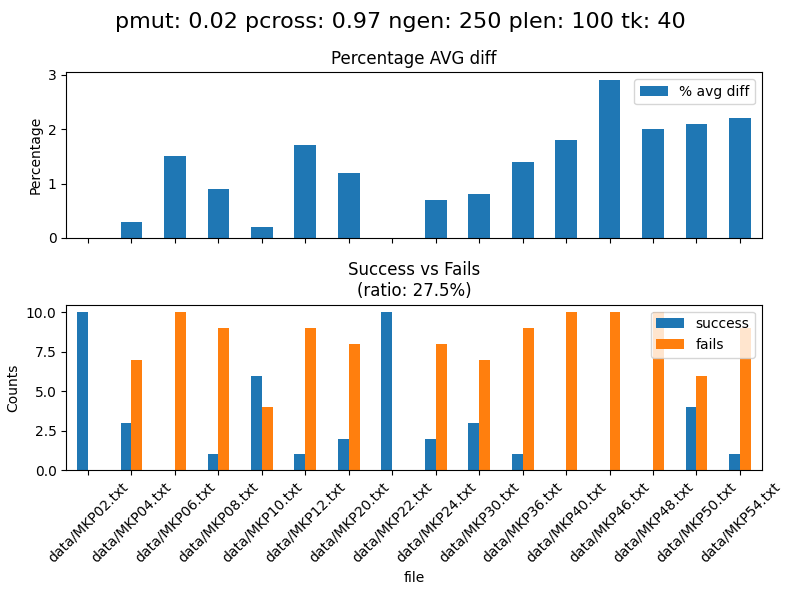
\includegraphics[width=\textwidth]{img/eval/evaluation_results_2_97_250_100_40.png}
    \end{subfigure}
    \begin{subfigure}{.49\textwidth}
        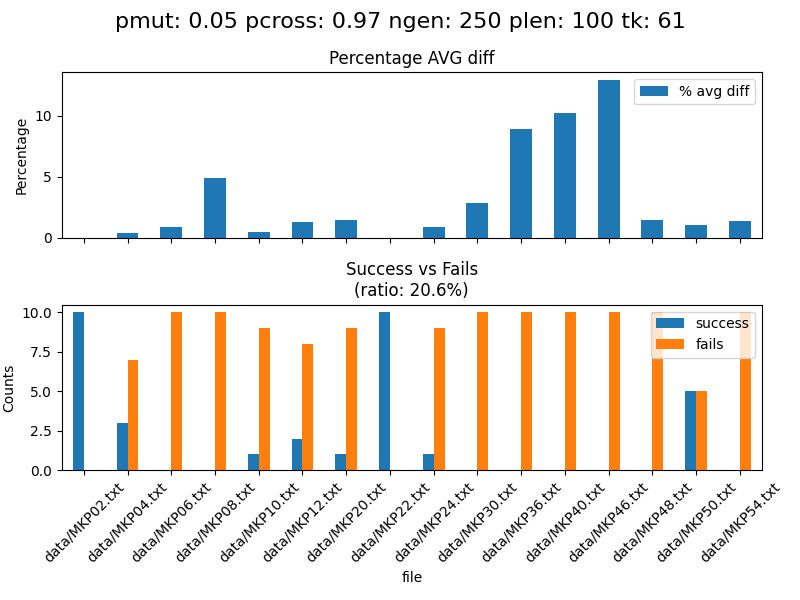
\includegraphics[width=\textwidth]{img/eval/evaluation_results_5_97_250_100_61.png}
    \end{subfigure}\\

    \begin{subfigure}{.5\textwidth}
        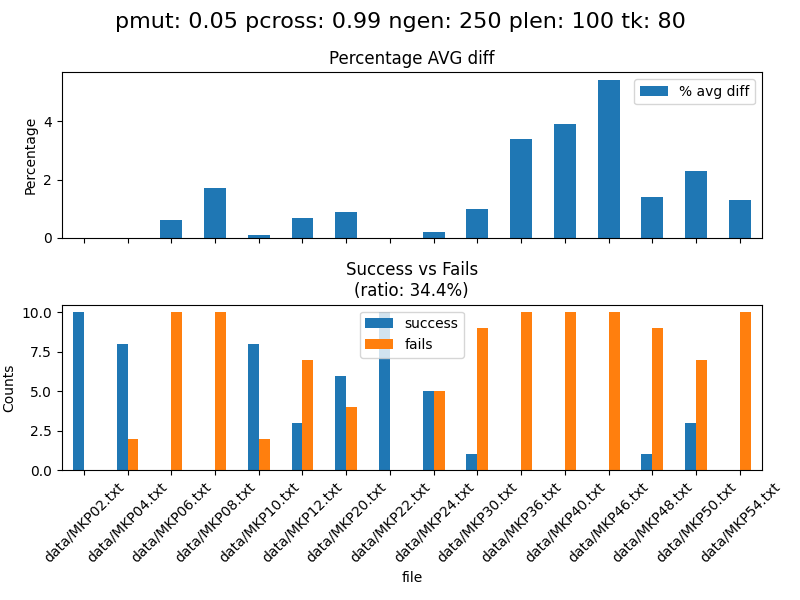
\includegraphics[width=\textwidth]{img/eval/evaluation_results_5_99_250_100_80.png}
    \end{subfigure}

    \caption{Grafici ottenuti dalla fase di Tuning.}
\end{figure}
